To be able to identify relationships within a changing urban form TOTUS
requires a route-able spatial road network, output from a traffic model
and demographic information. Exposure and energy demand information is
derived using these data sources.

\begin{figure}[h]
 \centering
 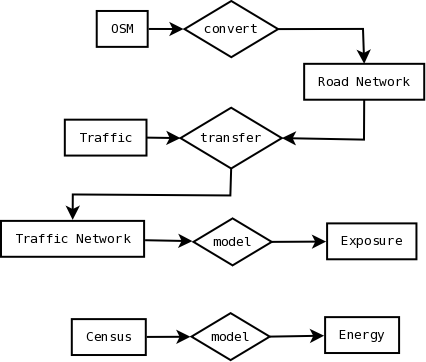
\includegraphics[scale=0.4,keepaspectratio=true]{./system_data.png}
 % system_data.png: 426x362 pixel, 51dpi, 21.30x18.10 cm, bb=0 0 604 513
\end{figure}


\subsection{OpenStreetMap}
OSM is used as the primary data source for TOTUS. It was chosen because
of its data coverage, it is open data license (released under the Open
Data Commons Open Database License) and its generic database schema
which is flexible and can store virtually any spatial datasets. In
addition for New Zealand it contains the Land Information New Zealand
(LINZ) datasets.

TOTUS uses the simple schema representation of the OSM data model, as
required by the OSM planet file loader.

\begin{figure}[h]
 \centering
 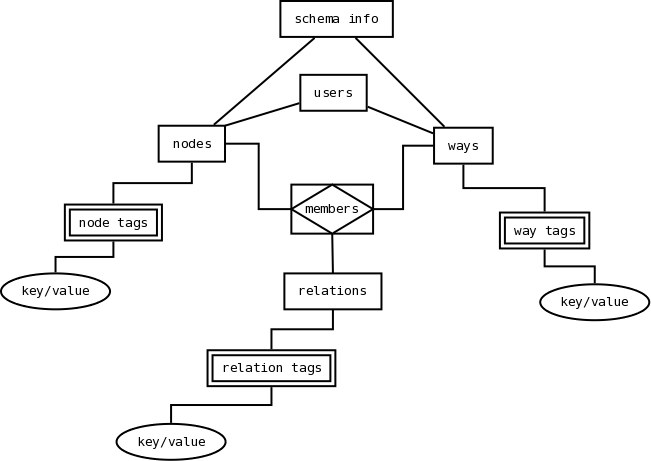
\includegraphics[scale=0.4,keepaspectratio=true]{./osm.png}
 % osm.png: 651x461 pixel, 51dpi, 32.55x23.05 cm, bb=0 0 923 653
\end{figure}


The OSM simple data model is an Entity-Attribute-Value (EAV) model with
post-ingestion validation. It constructs spatial features from nodes
and ways and has the ability to store relationships between map
features.

A node is the atomic element in the OSM data schema and used to
construct all linear features. It holds the only geometry needed by OSM
to represent linear map features and may or may not have any
attributes. Attribute are stored as an extensible list in what is a EAV
representation of spatial features. Nodes are allowed to be stranded
(isolated from road network) when marked as an amenity (a Point Of
Interest), but are usually the constituent parts of a spatial feature.

The \textit{node} table is one of the three data primitive
tables in the OSM physical model. It holds all the information needed
to identify a vertex and revision it's changes. The
OSM simple schema used by TOTUS only stores the most recent version of
all data primitives. Node attributes are stored in the
\textit{node\_tags} table as an extensible set of attribute
type/value pairs that can hold any attribution associated with the
vertex, eg. a roundabout, amenity, etc. Most nodes only exist to
describe ways, however they may still have attributes that provided
more information about the linear feature they are part of.

A way identifies any linear map features, eg. a road, ferry route,
railway line, cycle way, tramping track, area, etc. Polygon features
are represented as closed ways, but multi-polygons features can only be
represented using relations, eg. relationship amongst all
it's constituent area features. The
\textit{ways} table hold all the version and user
information, as well as (for convenience) the PostGIS geometry
constructed from the way's children node geometry. The
\textit{way\_nodes} store the link between a single way and
its constituent vertices. As a linear feature a way must have at least
2 bounding nodes. Each node has a sequence position within the way
which is used to maintain digitisation direction. The extensible list
of way attribution are stored as generic key value pairs in
\textit{way\_tags}. Although any properties can be stored
here, OSM encourages a standard way of denoting tags to allow for
interoperability of tools using OSM data.

Relations are used to construct complex features from nodes, ways or
even other relations and may be used to represent entities, eg. turn
restrictions. Relations may group related features together, eg. public
transport route. A relation consist of a feature or relation members,
each with it's own role in the relation. As with other
primitives relations may have an arbitrary number of attribute tags.
The relation's version and user information is stored
in \textit{relations}, the data primitives that are members
of the relation are stored in \textit{relation\_members} and
any attribution associated with the relation, eg. public transport
route number is present in \textit{relation\_tags}.

The OSM simple schema contains meta data that assist in re-visioning the
content and structure of the simple schema. This information is
dependent on by the schema objects and OSM planet file loader when
loading data to the target schema. This allows the loader to support
incremental data loads and use the revision history to only update the
records affected in a change set. The meta data include
\textit{users} which hold the OSM users that have made
changes to loaded dataset. OSM revisions all changes made to data
primitives and their attribution, however OSM simple does not hold any
historical data, only the latest. \textit{schema\_info}
holds the version number of the OSM simple schema, which allows the OSM
loader to know which schema to target when loading the data.

The current version of TOTUS is deployed on the Auckland region and
utilises the OSM data for Auckland only.

\subsection{Network}
The OSM simple schema data is not suitable for network routing. By
nature it is topological, but not necessary planar and cannot be
effectively used by \textit{pgRouting}. TOTUS uses the
\textit{pgRouting} OSM importer to create the correct planar
network topology from an OSM planet file. This utility depends on a
configuration file to load only the network classes TOTUS is interested
in for routing purposes. The network schema is created from the same
OSM planet XML file as imported into the OSM schema.

TOTUS uses a slighly modified version of
\textit{pgRouting}'s topological network
schema for OSM data, as created by their OSM importer.

\begin{figure}[h]
 \centering
 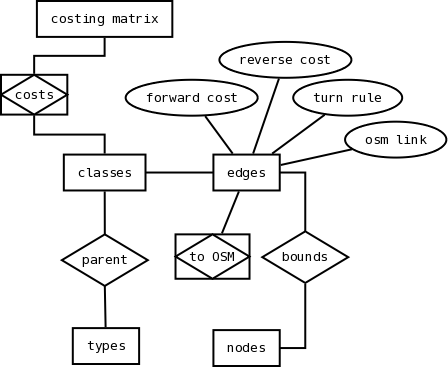
\includegraphics[scale=0.4,keepaspectratio=true]{./network.png}
 % network.png: 448x368 pixel, 51dpi, 22.40x18.40 cm, bb=0 0 635 522
\end{figure}


The \textit{types} and \textit{classes} classify
the network edges into network types, eg. highway, each with their own
classes, eg. motorway. This information is used by the routing
functions to consider only sub-networks, eg. only highway classes when
calculating routes and to apply rudimentary costing to the traversal of
an edge. The \textit{types} are the top level map feature
types in the OSM data set and TOTUS only import cycleway, highway,
junction and track type. The \textit{classes} are the
individual classes for the network types taken from the attribute
values in the OSM map feature keys and used to scale the cost of
traversing the network edges belonging to a specific network class.

In addition, TOTUS applies rudimentary costing per road class based on a
route mode option. The calling route function needs to specify the
route costing options to apply per road class to prevent certain road
types, not allowed by the mode of transport, to be considered as a
candidate edge, eg. cycling not allowed on motorway therefore the
motorway road class is allocated a very high course to deter cycling on
the motorway. The \textit{costing\_options} table holds the
information for the costing options which include distance only,
pedestrian, cycle and vehicle routing. The
\textit{class\_costs} holds the cost matrix for the
different classes for each route option. The cost itself is used as a
scaling factor to the base cost of traversing the edge.

The topological information is stored in \textit{nodes} and
\textit{edges}. The \textit{nodes} table contain
the vertices of the directed graph which bounds a graph edge. The
\textit{edges} table holds all the information needed for
\textit{pgRouting} which include the network class the edge
belongs to, it's great-circle distance length, the
name of the road the edge is part of, the start and end locations of
the edge which is used by A-star's heuristic filter, a
cost for traversing the edge in reverse, a turn restriction rule
implemented as a list of subsequent edges to follow, the cost of the
final edge in the turn restriction and the bounding source and target
nodes. The length of the edge is used as the default cost for
traversing the edge from source to target node, whilst the reverse cost
is used for going from target to source node. One
way's have a direction of flow from source to target
node and are assigned a huge reverse cost to prevent navigating through
it's target node against traffic flow.

\subsection{Traffic model}
The traffic model schema was designed to hold all traffic data as an
extensible set per link and to represent traffic routes.

\begin{figure}[h]
 \centering
 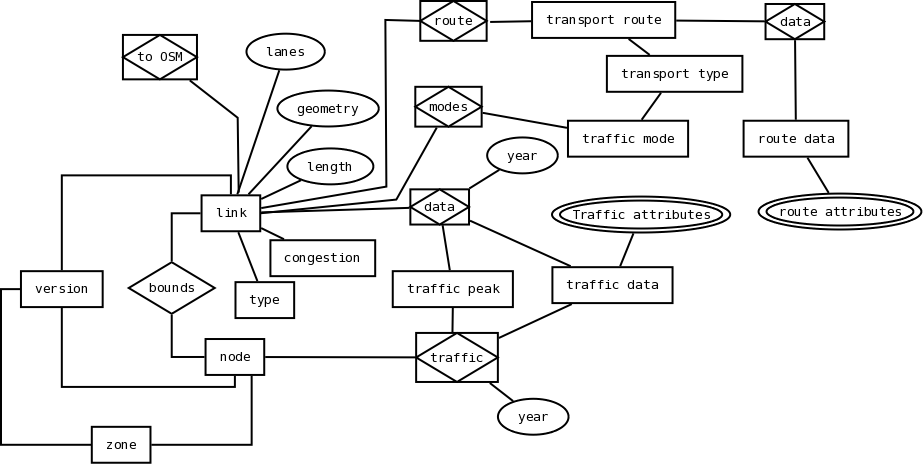
\includegraphics[scale=0.4,keepaspectratio=true]{./traffic_model.png}
 % traffic_model.png: 924x464 pixel, 51dpi, 46.20x23.20 cm, bb=0 0 1310 658
\end{figure}


TOTUS is deployed on Auckland and uses the Auckland Region Council
(ARC)'s EMME model output as traffic model. The
ARC's EMME provides a modelled view of traffic flow
through topological network links, which is an abstracted view of the
real network and may not correspond to the OSM road network features
and needs to be transferred manually.

The traffic data model of TOTUS needed to support different versions of
the same model run for the same year, same model runs for different
years with same or different link topology and same or different
traffic attributes. In addition it needed to support predetermined
grouping of modelled links as routes, eg. public transport routes,
freight routes, etc. The data schema was designed with these
requirements in mind.

At the core of the traffic model schema we have the topological modelled
links, their model meta data, transport modes and the model zones.

The lookup table \textit{link\_types} contains the road types
of the modelled links, which may or may not correspond to the OSM map
feature types. Any relationships between these road types and OSM ones
are used in transferring traffic model links to OSM network edges. The
\textit{congestion\_function} is model specific and hold
information about the different congestion functions applied to the
links during modelling. The different transport modes supported by a
modelled link for which the traffic flow is relevant is stored in
\textit{transport\_mode}. The transport modes may include
bus, rail, ferry, etc. Some traffic models classify the modelled links
into zones and apply inter-zone modelling as well, these are filtered
from TOTUS, but the information about the modelled areas are stored in
\textit{zones}.

The \textit{link} table contains topological, version and
physical attribution about the modelled geometry. The attribution
include the length of the roads modelled by this link, the number of
lanes simulated and the congestion function applied. The
\textit{node} data is created from the modelled links,
unless provided. Each link may have traffic data modelled for multiple
transport modes; the \textit{link\_transport\_mode} relates
a link to all it's transport modes.

The traffic model provides an extensible set of traffic attributes for
each link for different traffic peaks, eg. morning, inter and evening
peak. The lookup table \textit{traffic\_peak} contains the
definition for each traffic peak and allows defining custom profiles.
\textit{traffic\_attribute} defines a traffic attribute, eg.
link traversal time, total vehicles per 2hr, and provides information
on how to interpret such an attribute by defining it's
data type. Traffic attributes may different from one model and/or year
run to the next and may not always be present and each have a version.

The \textit{traffic\_data} tables holds the actual instances
of the traffic attributes, eg. the attribute values for the defined
traffic attributes types. This table contains unique attribute value
pairs and is fully normalised.\textit{link\_traffic\_data}
links an traffic model geometry link to all instances of its traffic
attributes for each traffic peak and model year, whereas
\textit{node\_traffic\_data} store any traffic data present
for the link nodes.

Another purpose of the traffic data model is to store model information
for transport routes. Tables have been defined to represent a modelled
view of transport routes, eg. public or freight routes, which consist
of a sequence of traffic model links and holds the route
link's attributes, eg. number of public transport
routes allocated. The route itself may also have attributes, eg. like 1
ton trucks only. \textit{route\_attribute} define a
pre-linked route attribute definition, whereas
\textit{route\_data} hold the instance data for a route
attribute.

Each transport route are associated with a type of transport and consist
of a type, eg. public, a transport mode, eg. rail, a vehicle, eg. train
and a description. These are stored in
\textit{transport\_type}.
\textit{transport\_route} describes the route itself and
contains route identifier, description and transport type information;
\textit{transport\_route\_data} links a route to all of its
transport attributes and \textit{transport\_route\_link}
which defines the route path usig the the traffic model links (in
order) that makes up the pre-linked path.

As mentioned earlier the traffic model output may not always correspond
to the real work and TOTUS may require a mechanism of relating an
traffic model link to one or more OSM network edges. Each OSM network
edge assigned to an traffic model link is allocated a fraction of the
traffic flow of the traffic model link. This information is used mostly
for aggregated traffic model traffic information on a sub-network, a
dynamic route, eg. pupil trip to school, etc.
\textit{link\_network} relates an traffic model link with
one or more OSM network edges and is vital in aggregating traffic model
output derived variables, such as the Traffic Impact Factor (TIF).

Lastly the traffic data model holds meta data about the versions of the
traffic model and transport model, as well as the year of the data used
in model run. This information is stored in
\textit{version}.

\subsection{Demographic}
TOTUS relies on demographic information at the mesh block level for
deriving energy related variables by producing simple energy models.
Auckland TOTUS uses Statistics New Zealand's census
dataset. Census data is provided as a collection of data sets for each
instance of an administration area (geographies). For New Zealand these
are mesh block, area unit, ward, territorial authority and regional
council.

The administrative hierarchy is represented as a tree with each level of
a specific administrative type. Demographic data is assigned to the
mesh blocks only since each higher administrative level can determine
their census data using aggregation. In general Census data is provided
as a collection of data per topic. Each topic has a set of categories,
each with it's own set of classifications. The
demographic information is assigned to the class. These aspects are all
incorporated in the design of the demographic data model.

\begin{figure}[h]
 \centering
 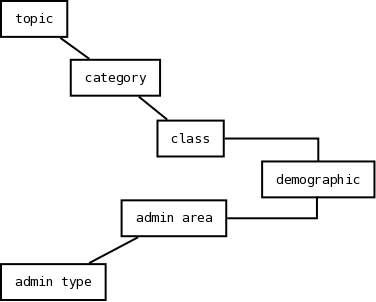
\includegraphics[scale=0.4,keepaspectratio=true]{./census.png}
 % census.png: 376x302 pixel, 51dpi, 18.80x15.10 cm, bb=0 0 533 428
\end{figure}


The demographic data schema in TOTUS defines the administrative types or
levels of the area hierarchy in the table
\textit{admin\_type} and stores the actual administrative
areas in \textit{admin\_area}. The administrative areas are
defined within an administrative or geographic hierarchy, but do allow
for non-hierarchical data as well when its parent administrative place
is missing. The census topics include about people, households, etc.
and stored as a lookup list in \textit{topic}. Similarly
\textit{category} stores the category for a given topic, eg.
age in 5 year groups and \textit{class} holds the different
classes for a category, eg. 0 - 4 years. The
\textit{demographic} table holds the instance of a statistic
of the human population, which is the tally per demographic class.